% !TEX program = xelatex
\documentclass[tikz, crop, border = {2pt 2pt 2pt 2pt}]{standalone}

\usepackage{concmath-otf}
\usetikzlibrary{calc, angles, quotes, patterns}
\usetikzlibrary{decorations.pathreplacing, decorations.pathmorphing, calligraphy}

\begin{document}
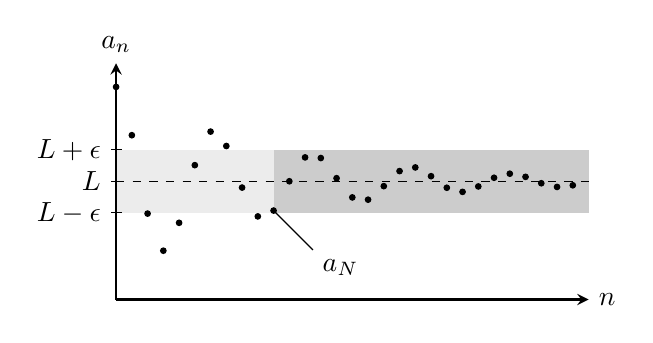
\begin{tikzpicture}
	\def\tol{0.4}
	\def\ix{2.0}
	\fill[lightgray!30] (0, {1.5 + \tol}) rectangle (6, {1.5 - \tol});
	\fill[lightgray!80] (\ix, {1.5 + \tol}) rectangle (6, {1.5 - \tol});
	\draw[-stealth, thick] (0, 0) -- (6, 0) node[right]{$n$};
	\draw[-stealth, thick] (0, 0) -- (0, 3) node[above]{$a_n$};

	\foreach \i [count = \xi] in {0, 0.2, 0.4, ..., 5.8} {
			\filldraw (\i, {1.2*cos(5*\i r) * e^(-0.5*\i) + 1.5}) circle (1pt);
		}

	\node (aN) at (\ix, {1.2*cos(5*\ix r) * e^(-0.5*\ix) + 1.5}){};
	\draw ($(aN.center)$) -- ++ (0.5, -0.5) node[below right]{$a_N$};

	\draw[dashed] (0, 1.5) -- ++ (6, 0);

	\draw (2pt, 1.5) -- ++ (-4pt, 0) node[left]{$L$};
	\draw (2pt, {1.5 + \tol}) -- ++ (-4pt, 0) node[left]{$L + \epsilon$};
	\draw (2pt, {1.5 - \tol}) -- ++ (-4pt, 0) node[left]{$L - \epsilon$};
\end{tikzpicture}
\end{document}
